\chapter{Computer Code}
\label{ch:code}
Critical for being able to reproduce the result of any analysis presented in this thesis is knowledge of the computer code used to analyse the data.
This section contains the code used to analyse data and create synthetic data sets for the \ac{dvc}.
Each section contains a link to an on-line version of the code, hosed at GitHub (\url{http://www.github.com}).
Any changes made to the code after publication of this thesis will be available on GitHub.

\section{Drop tower and Instron analysis}
\label{sec:code_dt_ins_analysis}
This section contains the MatLab code used to analyse the fall simulator and Instron data.
All of the code, except for the example input (\S\ref{sec:code_dt_ins_analysis_example}), can be found at \url{https://github.com/sethgilchrist/DroptowerInstronAnalysis}.

The tests in the fall simulator and Instron generated huge amounts of data.
The organization and analysis of this data was standardized through the use of classes for each dataset, test and specimen.
There are eight classes in each experiment (Figure~\ref{fig:AnalysisHigherarchy}).
The Instron test contains a \ac{dic} dataset, a \ac{daq} dataset and a link to the specimen associated with the experiment.
The drop tower test contains a \ac{dic} dataset, a \ac{daq} dataset, a displacement dataset and a link to the specimen associated with the experiment.
Note that due to different data begin collected in the Instron \ac{daq} dataset than the drop tower \ac{daq} dataset, these are two different classes.

\begin{figure}
\centering
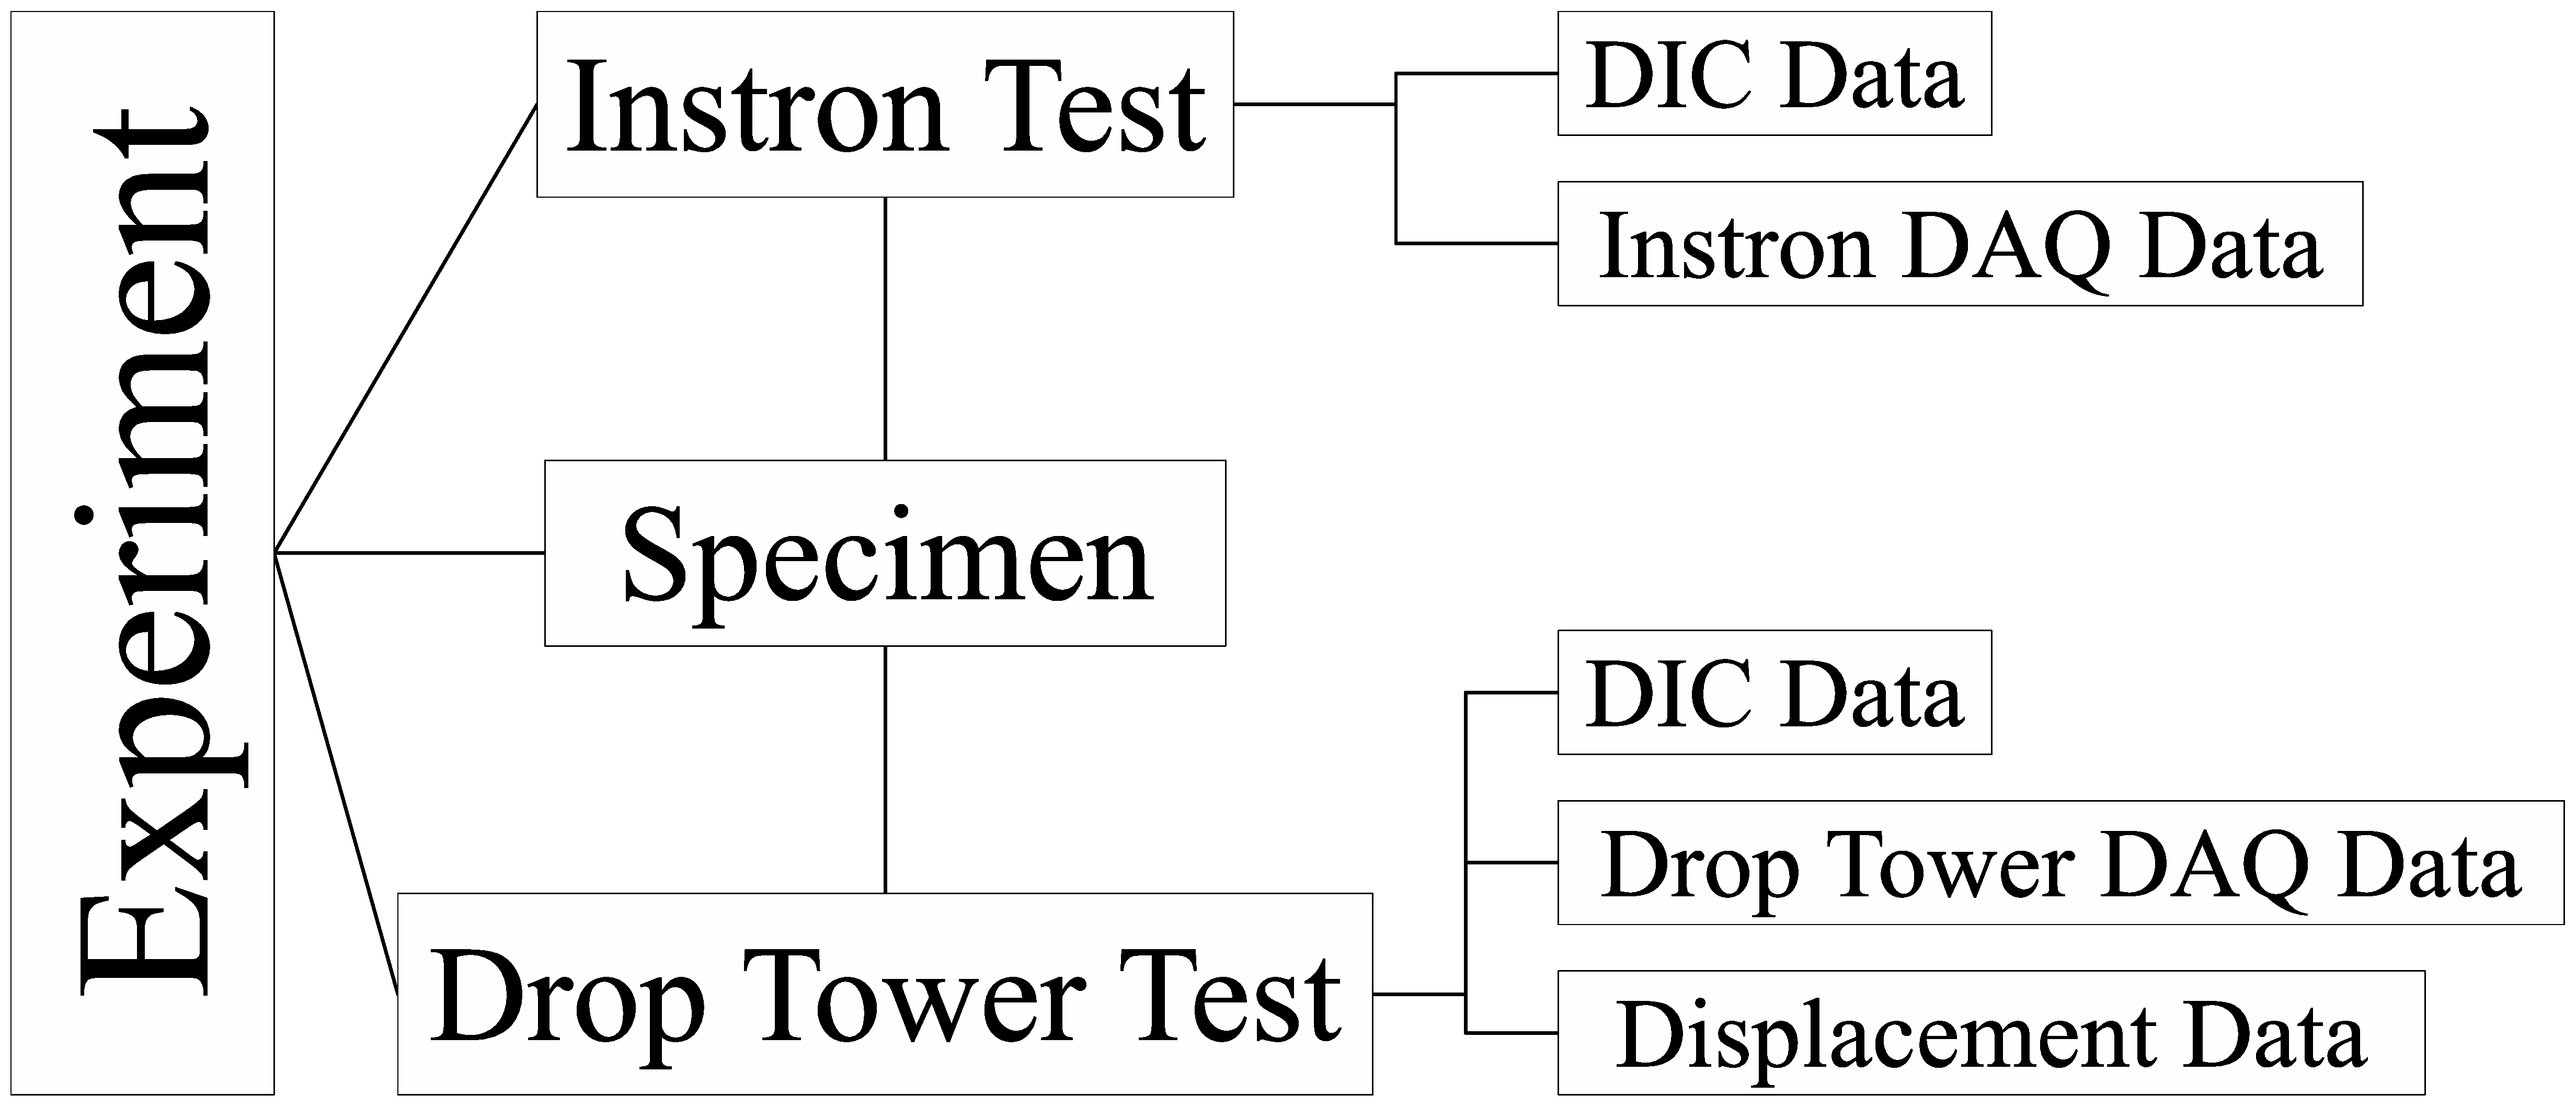
\includegraphics[width=\linewidth]{./appendixCode/analysisCode/Figures/AnalysisHigherarchy}
\caption[Data analysis hierarchy]{The hierarchy of the experimental data analysis. Each box is a Matlab class. Graphic \textcopyright Seth Gilchrist, 2013.}
\label{fig:AnalysisHigherarchy}
\end{figure}

The reason for implementing the code in this way was so that all details of a given analysis would be preserved, in one location, for later review.
If, for example, one wanted to know the filter order used to prepare the displacement data, this could found using the command 

\texttt{>> experiment.GetDropTower.GetDisplacement.GetFilterOrder()}.

Raw data, as well as analysed data, are also stored in the class.
In the end, saving the class object to disk allows for unified saving of all raw data, analysis routines and analysed data in a single \ac{mat}.
 
The code for each of these data analysis classes are given below.
Documentation is built into the MatLab files, so once they are placed in the current MatLab directory or path, help can be found by typing ``\texttt{help <Class Name>.<Method Name>}" at the command line.
Alternatively, all methods are documented in the code.

\subsection{Example input}
\label{sec:code_dt_ins_analysis_example}
Assuming that the data for the desired analysis are stored in ``C:\textbackslash Data\textbackslash TestData\textbackslash", an analysis can be carried out using the following code.
\begin{singlespace}
\begin{lstlisting}
% Fill in the specimen data
name = 'specimen01';
gender = 'm';
age = 80;
height = 170;
weight = 60;
dxa = struct('neck',0.67,'troch',.70,'inter',.70,'total',.75,'wards',0);
op = 'osteopenia';
data = struct('InstronDAQ',1,'InstronDIC',1,'DropTowerDAQ',1,'DropTowerDisplacement',1,'DropTowerDIC',1);

% create the specimen object
specimen = Specimen(name,gender,age,height,weight,dxa,op,data);

% create the experiment object. All sub-objects (DAQ analyses, etc) will be created based on the data structure.
experiment = Experiment(specimen);

% Get the Instron analysis
instronAnalysis = experiment.GetInstron();

% Setup the Instron DAQ parameters
instronAnalysis.GetDAQData.SetFileName('C:\Data\TestData\InstronDAQ.csv');
instronAnalysis.GetDAQData.ReadFile();

instronAnalysis.GetDAQData.SetSampleRate(20000);
instronAnalysis.GetDAQData.SetFilterCutoff(500);
instronAnalysis.GetDAQData.SetGainDisplacement(.35);
instronAnalysis.GetDAQData.SetGainLoad(1200);

% Setup the Instron DIC
instronAnalysis.GetDICData.SetFileName('C:\Data\TestData\InstronDIC.csv');
instronAnalysis.GetDICData.ReadFile();

instronAnalysis.GetDICData.SetSampleRate(100)
instronAnalysis.GetDICData.SetStartTime(0.85)

% Get the drop tower analysis
dropTowerAnalysis = experiment.GetDropTower();

% Setup the drop tower DAQ
dropTowerDAQ = dropTowerAnalysis.GetDAQData();
dropTowerDAQ.SetFileName('C:\Data\TestData\DropTowerDAQ.csv');
dropTowerDAQ.ReadFile();

dropTowerDAQ.SetExcitation(12);
dropTowerDAQ.SetSampleRate(20000);
dropTowerDAQ.SetFilterCutoff(500);
dropTowerDAQ.SetFilterOrder(4);

% Setup the drop tower displacement
dropTowerDisp = dropTowerAnalysis.GetDisplacementData();
dropTowerDisp.SetFileName('C:\Data\TestData\DropTowerDAQ.csv');
dropTowerDisp.ReadFile();

dropTowerDisp.SetSampleRate(9600);
dropTowerDisp.SetFilterCutoff(500);
dropTowerDisp.SetTimeStart(-0.05);
dropTowerDisp.SetFilterOrder(2);

% Setup the drop tower DIC
dropTowerDIC = dropTowerAnalysis.GetDICData();
dropTowerDIC.SetFileName('C:\Data\TestData\DropTowerDIC.csv');
dropTowerDIC.ReadFile();

dropTowerDIC.SetStartTime(-.03);
dropTowerDIC.SetSampleRate(10000);

% Run the analysis
experiment.update(1);

% Save the resulting data
save('C:\Data\TestData\Specimen01.mat','experiment');
\end{lstlisting}
\end{singlespace}
\begin{singlespace}
\subsection{Specimen class}
\input{appendixCode/analysisCode/specimenClass}

\subsection{Experiment class}
\input{appendixCode/analysisCode/experiment}

\subsection{Instron test class}
\input{appendixCode/analysisCode/instronTestClass}

\subsection{Instron \acs*{daq} class}
\input{appendixCode/analysisCode/instronDaqClass}

\subsection{Drop tower test class}
\input{appendixCode/analysisCode/dropTowerTestClass}

\subsection{Drop tower \acs*{daq} class}
\input{appendixCode/analysisCode/dropTowerDaqClass}

\subsection{Drop tower displacement class }
\input{appendixCode/analysisCode/displacementClass}

\subsection{\acs*{dic} data class}
\input{appendixCode/analysisCode/dicClass}
\end{singlespace}

\section{Idealized fall simulator model}
\label{sec:code_ideal_fs}
The idealized model discussed in \S\ref{sec:behave_fail_discssion} was solved using MatLab (R2010b, The Mathworks, Natick, MA).
Code used to solve the equations and create the plots is given below.
The code contained herein is available for download from\newline \url{https://github.com/sethgilchrist/IdealFallSimModel}.
\begin{singlespace}
\subsection{Solving the system \acs{ode}}
\label{sec:code_ideal_fs_ode}
\begin{lstlisting}
function [displacementRate,loadingRate] = stiffVsRatesData(kFemur,bFemur)
% This function takes a vector of femoral stiffnesses (length = s) and a 
% vector of femoral damping values (length = d) as inputs and returns two
% d by s matricies of displacement and loading rates. Each row corresponds
% to a damping value and each column to a stiffness value.

% define stiffnesses
kPlevis = 50000; %N/m

% preallocate
displacementRate = zeros(length(bFemur),length(kFemur));
loadingRate = zeros(size(displacementRate));

% solve the ode
for i = 1:size(displacementRate,1)
    for j = 1:size(displacementRate,2)
        % get the time and displacement values from the ODE solver
        [t,x] = displacementSimple(kFemur(j),kPlevis,bFemur(i));
        % find the first time that the compression and damping are greater
        % than 1500 N
        cIndex = find(x(:,3)*kFemur(j)+x(:,4)*bFemur(i) > 1500,1,'first')-1;
        % calculate the displacement rate
        displacementRate(i,j) = x(cIndex,3)/t(cIndex);
        % calculate the loading rate based on the average displacement rate
        % for the velocity of the compression
        loadingRate(i,j) = (x(cIndex,3)*kFemur(j) + bFemur(i)*displacementRate(i,j))/t(cIndex);
    end
end
end


function [t,x] = displacementSimple(kf,ks,bf)
% A simple model of the fall simulator consisting of two masses, two
% springs and one damper.
% Usage
% [t,x] = displacementSimple(femurStiffness,springStiffness,femurDamping)
%
% t = vector of time
% x(1) = displacement of top of spring
% x(2) = velocity of top of spring
% x(3) = displacement of trochanter
% x(4) = velocity of trochanter

springMass = 3.5; %kg

M1 = springMass/3 + 1 + 32; % kg: top 1/3 spring + top plate + body mass
M2 = springMass/3 + 10 + 1.98; %kg: bottom 1/3 spring + bottom plate + stabalizer + loadcell + loader +  falling mass

initialConditions = [0,2.9,0,0];

[t,x] = ode45(@(t,x) system(t,x,M1,M2,kf,ks,bf),linspace(0,0.05,5000),initialConditions);
end

function dxdt = system(t,x,M1,M2,Kf,Ks,Bf)
if t < 0.005
    f2pulse = 250*sin(2*pi/.01*t); % repace this line with "f2pulse = 0" to omit the force pulse on mass 2
else
    f2pulse = 0;
end

xM1 = x(1);
xM1dot = x(2);
xM2 = x(3);
xM2dot = x(4);

dxdt = zeros(size(x));
dxdt(1) = xM1dot;
dxdt(2) = 1/M1 * (9.81*M1 + (xM2-xM1)*Ks);
dxdt(3) = xM2dot;
dxdt(4) = 1/M2 * (9.81*M2 + f2pulse - xM2*Kf - (xM2-xM1)*Ks - xM2dot*Bf);
end
\end{lstlisting}


\subsection{Plotting the system response}
\label{sec:code_ideal_fs_plot}
\begin{lstlisting}
% house keeping
close all
clear all

% femur stiffness values to analyse
kFemur =  (.4:.25:4.5)*1000000; %N/m
% femur damping values to analyse
bFemur = [0 300 600 4000]; %Ns/m

% calculate the loading and displacement rates for the different
% stiffnesses and damping values
[disp,load] = stiffVsRatesData(kFemur,bFemur);

% create the figure
fH1 = figure(1);
set(fH1,'position',[463 29 1066 945],'paperpositionMode','auto');
for i = 1:4
    % calculate a subplot position
    aH = subplot(2,2,i);
    % plot and get plot object handles
    [aHyy(i,:),L1(i),L2(i)] = plotyy(kFemur/1000000,load(i,:)/1000,kFemur/1000000,disp(i,:)*1000); %#ok<*SAGROW>
    % move plotyy axes to the right place based on the subplot location
    oP = get(aH,'position'); % original position
    set(aHyy(i,1),'position',[oP(1)-.025 oP(2:4)],... % location
        'ycolor','k','fontname','times','fontsize',20,... % axes appearance
        'xlim',[0 5],'xtick',[0 1 2 3 4 5],... % x limits and ticks
        'ylim',[0 300],'ytick',[0 150 300]); % y limits and ticks
    
    set(aHyy(i,2),'position',[oP(1)-.025 oP(2:4)],... % location
        'ycolor','k','fontname','times','fontsize',20,... % axes appearance
        'xlim',[0 5],'xtick',[0 1 2 3 4 5],... % x limits and ticks
        'ylim',[0 400],'ytick',[0 200 400]); % y limits and ticks
    
    grid(aHyy(i,1)); % turn the grid on for one axes
    % set the data styles
    set(L1(i),'marker','o','markersize',10,'linestyle','none','markerEdgeColor','k','lineWidth',2)
    set(L2(i),'marker','x','markersize',10,'linestyle','none','markerEdgeColor','k','lineWidth',2)
    % calculate fit lines
    loadingFit(i,:) = polyfit(kFemur,load(i,:),1);
    dispFit(i,:) = polyfit(kFemur,disp(i,:),1);
    % plot the fit lines
    hold(aHyy(i,1))
    plot(aHyy(i,1),kFemur/1000000,polyval(loadingFit(i,:),kFemur)/1000,'--k','linewidth',2)
    hold(aHyy(i,2))
    plot(aHyy(i,2),kFemur/1000000,polyval(dispFit(i,:),kFemur)*1000,'--k','linewidth',2)
    % set the text with the damping values in the upper left corner
    damping = sprintf('%0.1f',bFemur(i)/1000);
    hText = text(.3,260,[damping ' $$\frac{N}{mm/s}$$'],'fontname','times','fontsize',25,'interpreter','latex','HorizontalAlignment','left','backgroundcolor','w');
end
% put axes labels in position
LyP = get(get(aHyy(3,1),'ylabel'),'position');
set(get(aHyy(3,1),'ylabel'),'string','Loading Rate (kN/s)','fontname','times','fontsize',30,'position',[LyP(1) 375 1])
BxP = get(get(aHyy(3,1),'xlabel'),'position');
set(get(aHyy(3,1),'xlabel'),'string','Stiffness (kN/mm)','fontname','times','fontsize',30,'position',[6 BxP(2) 1])
RyP = get(get(aHyy(4,2),'ylabel'),'position');
set(get(aHyy(4,2),'ylabel'),'string','Displacement Rate (mm/s)','fontname','times','fontsize',30,'position',[RyP(1) 500 1])

% put tips in the first plot to indicate which curves are loading and
% displacement.
set(fH1,'currentAxes',aHyy(1,1));
hLoading = text(3.15,225,'Loading','fontname','times','fontsize',20);
set(fH1,'currentAxes',aHyy(1,2));
hDisplace = text(2.5,50,'Displacement','fontname','times','fontsize',20,'HorizontalAlignment','right');

% save the plots as eps (for latex), png (for review) and fig (for easy editing)
print(fH1,'../ratesVsDamping.eps','-r300','-deps');
print(fH1,'ratesVsDamping.png','-r150','-dpng');
saveas(fH1,'ratesVsDamping.fig')
\end{lstlisting}


\end{singlespace}

\section{\acs*{dic} to \acs*{dic} registration and comparison}
\label{sec:code_dic_dic_register_compare}
This section contains \ac{cpp} code used to register two surfaces created by DaVis and transfer a single set of point-data from one to the other.
The code contained herein is available for download at \url{https://github.com/sethgilchrist/RegisterCompareDICSurfaces}.
\begin{singlespace}


\subsection{Functions library for converting DaVis to \acs*{vtk} format}
\label{sec:code_dic_dic_convertLib}
Header file:
\begin{lstlisting}
//      ReadInputFiles.h
//
//      Copyright 2011 Seth Gilchrist <seth@sethgilchrist.com>
//
//      This program is free software; you can redistribute it and/or modify
//      it under the terms of the GNU General Public License as published by
//      the Free Software Foundation; either version 3 of the License, or
//      (at your option) any later version.
//
//      This program is distributed in the hope that it will be useful,
//      but WITHOUT ANY WARRANTY; without even the implied warranty of
//      MERCHANTABILITY or FITNESS FOR A PARTICULAR PURPOSE.  See the
//      GNU General Public License for more details.
//
//      You should have received a copy of the GNU General Public License
//      along with this program; if not, write to the Free Software
//      Foundation, Inc., 51 Franklin Street, Fifth Floor, Boston,
//      MA 02110-1301, USA.

#ifndef READDAVIS_H
#define READDAVIS_H


#include <cstring>
#include <sstream>
#include <iterator>
#include <boost/tokenizer.hpp>
#include <vtkSmartPointer.h>
#include <vtkPointData.h>
#include <vtkPolyData.h>
#include <vtkImageData.h>
#include <vtkDoubleArray.h>
#include <vtkDelaunay2D.h>


class ReadDaVis
{
public:

    /** Constructor **/
    ReadDaVis();

    /** Set/Get the height file name.**/
    void SetHeightFileName( std::string fileName );
    std::string GetHeightFileName();
    /** Set the strain file name. **/
    void SetStrainFileName( std::string fileName );

    /** Read the height file **/
    void ReadHeightFile();
    /** Read the strain file **/
    void ReadStrainFile();
    /** Read a file given in fileName and put the results in the pointset **/
    void ReadFile(std::string fileName, vtkSmartPointer<vtkImageData> pointData);
    /** Put the height data into a surface and put the z-comp of the strain
      * point data as a dataset at the points of the hight data. **/
    void CreateDataSurface();

    /** Get the height point data. **/
    vtkSmartPointer<vtkImageData> GetHeightData();
    /** Get the strain point data. **/
    vtkSmartPointer<vtkImageData> GetStrainData();
    /** Get the surface. **/
    vtkSmartPointer<vtkPolyData> GetSurface();
    //vtkSmartPointer<vtkUnstructuredGrid> GetSurface();


private:
    std::string                                 m_heightFileName;
    std::string                                 m_strainFileName;
    vtkSmartPointer<vtkImageData>               m_heightData;
    vtkSmartPointer<vtkImageData>               m_strainData;
    vtkSmartPointer<vtkPolyData>                m_surface;
    //vtkSmartPointer<vtkUnstructuredGrid>        m_surface;

};
#endif
\end{lstlisting}

C++ file:
\begin{lstlisting}
//      ReadDaVis.cpp
//
//      Copyright 2011 Seth Gilchrist <seth@sethgilchrist.com>
//
//      This program is free software; you can redistribute it and/or modify
//      it under the terms of the GNU General Public License as published by
//      the Free Software Foundation; either version 3 of the License, or
//      (at your option) any later version.
//
//      This program is distributed in the hope that it will be useful,
//      but WITHOUT ANY WARRANTY; without even the implied warranty of
//      MERCHANTABILITY or FITNESS FOR A PARTICULAR PURPOSE.  See the
//      GNU General Public License for more details.
//
//      You should have received a copy of the GNU General Public License
//      along with this program; if not, write to the Free Software
//      Foundation, Inc., 51 Franklin Street, Fifth Floor, Boston,
//      MA 02110-1301, USA.

#include "ReadDaVis.h"

/** Constructor **/
ReadDaVis::ReadDaVis()
{
//    m_heightFileName; // Must be provided by user
//    m_strainFileName; // Must be provided by user
m_heightData  = vtkSmartPointer<vtkImageData>::New();
m_strainData  = vtkSmartPointer<vtkImageData>::New();
m_surface     = vtkSmartPointer<vtkPolyData>::New();
//m_surface       = vtkSmartPointer<vtkUnstructuredGrid>::New();
}

void ReadDaVis::SetHeightFileName( std::string fileName )
{
    if (m_heightFileName.compare(fileName) != 0) {m_heightFileName = fileName;}
}
std::string ReadDaVis::GetHeightFileName()
{
    return m_heightFileName;
}

void ReadDaVis::SetStrainFileName( std::string fileName )
{
    if (m_strainFileName.compare(fileName) != 0) {m_strainFileName = fileName;}
}

void ReadDaVis::ReadHeightFile()
{
    ReadFile(m_heightFileName,m_heightData);
}

void ReadDaVis::ReadStrainFile()
{
    ReadFile(m_strainFileName,m_strainData);
}

void ReadDaVis::ReadFile(std::string fileName, vtkSmartPointer<vtkImageData> pointData)
{
    // create a stringstream for passing info to the user
    std::stringstream msg(" ");
    // open the file
    std::ifstream inFile(fileName.c_str());
    if (!inFile){
        msg.str(" ");
        msg << "Cannot open\n" <<fileName<<"\nPlease check the name and try again."<<std::endl;
        std::cout << msg;
    }

    // Get the header line
    std::string headerLine;
    std::getline(inFile,headerLine);
    std::vector<std::string> headerTokens;
    boost::char_separator<char> sep(" ");
    boost::tokenizer< boost::char_separator<char> > tok(headerLine,sep); // the boost library tokenizer
    for (boost::tokenizer< boost::char_separator<char> >::iterator beg=tok.begin(); beg!=tok.end();++beg){
        headerTokens.push_back(*beg);
    }

    int xDimension = atoi(headerTokens[3].c_str());
    float xScale = atof(headerTokens[6].c_str());
    float xOffset = atof(headerTokens[7].c_str());
    int yDimension = atoi(headerTokens[4].c_str());
    float yScale = atof(headerTokens[10].c_str());
    float yOffset = atof(headerTokens[1].c_str());
    pointData->SetDimensions(xDimension,yDimension,1);
    pointData->SetOrigin(xOffset,yOffset,0);
    pointData->SetSpacing(xScale,yScale,1);

    // now step through the file and create the points
    std::string cline;
    unsigned int i = 0; // the x point number, will be used with x-scale and x-offest to produce an point

    while( std::getline (inFile,cline))
    {
        // break the current line into values of height
        std::vector<double> values;
        boost::tokenizer< boost::char_separator<char> > tok(cline,sep);
        for (boost::tokenizer< boost::char_separator<char> >::iterator beg=tok.begin(); beg!=tok.end();++beg)
        {
            std::string current = *beg;
            values.push_back(atof(current.c_str()));
        }
        for (int j = 0; j < yDimension; ++j)
        {
            pointData->SetScalarComponentFromDouble(i,j,0,0,values[j]);
        }
        ++i;

    }
    inFile.close();

}

void ReadDaVis::CreateDataSurface()
{
    // find out which point set has fewer points
    int* heightDimensions = m_heightData->GetDimensions();
    int* strainDimensions = m_strainData->GetDimensions();
    int xEnd = (heightDimensions[0] > strainDimensions[0]) ? strainDimensions[0] : heightDimensions[0];
    int yEnd = (heightDimensions[1] > strainDimensions[1]) ? strainDimensions[1] : heightDimensions[1];

    vtkSmartPointer<vtkPoints>  surfacePoints = vtkSmartPointer<vtkPoints>::New();
    vtkSmartPointer<vtkDoubleArray> surfaceArray = vtkSmartPointer<vtkDoubleArray>::New();
    surfaceArray->SetNumberOfComponents(1);
    surfaceArray->SetName("MinPStrain");

    // iterate through x and y, if the data for both != 0, then save the point
    for (int i = 0; i<xEnd; ++i)
    {
        for (int j = 0; j< yEnd; ++j)
        {
            double heightPoint = m_heightData->GetScalarComponentAsDouble(i,j,0,0);
            double strainPoint = m_strainData->GetScalarComponentAsDouble(i,j,0,0);
            if (heightPoint!=0 && strainPoint!=0)
            {
                int pointIndex[3];
                pointIndex[0] = i;
                pointIndex[1] = j;
                pointIndex[2] = 0;
                double* pointLocation = m_heightData->GetPoint(m_heightData->ComputePointId(pointIndex));
                surfacePoints->InsertNextPoint(pointLocation[0],pointLocation[1],heightPoint);
                surfaceArray->InsertNextTuple1(strainPoint);

            }

        }
    }

    m_surface->SetPoints(surfacePoints);
    m_surface->GetPointData()->AddArray(surfaceArray);

    // use Delaunay2D to create a mesh, ignoring the z-dimension
    vtkSmartPointer<vtkDelaunay2D> delauney = vtkSmartPointer<vtkDelaunay2D>::New();
    delauney->SetInput(m_surface);
    delauney->Update();
    m_surface = delauney->GetOutput();

}

vtkSmartPointer<vtkImageData> ReadDaVis::GetHeightData()
{
    return m_heightData;
}

vtkSmartPointer<vtkImageData> ReadDaVis::GetStrainData()
{
    return m_strainData;
}

vtkSmartPointer<vtkPolyData> ReadDaVis::GetSurface()
{
    return m_surface;
}
\end{lstlisting}
		

\subsection{Main program for converting output from DaVis to \acs*{vtk} format}
\label{sec:code_dic_dic_convert}
\begin{lstlisting}
/*
* ConvertSurfaces.cpp
*
* Copyright 2013 Seth Gilchrist <seth@sethgilchrist.com>
*
* This program is free software; you can redistribute it and/or modify
* it under the terms of the GNU General Public License as published by
* the Free Software Foundation; either version 3 of the License, or
* (at your option) any later version.
*
* This program is distributed in the hope that it will be useful,
* but WITHOUT ANY WARRANTY; without even the implied warranty of
* MERCHANTABILITY or FITNESS FOR A PARTICULAR PURPOSE.  See the
* GNU General Public License for more details.
*
* You should have received a copy of the GNU General Public License
* along with this program; if not, write to the Free Software
* Foundation, Inc., 51 Franklin Street, Fifth Floor, Boston,
* MA 02110-1301, USA.
*
*
*/

#include "../lib/ReadDaVis/ReadDaVis.h"
#include <vtkIterativeClosestPointTransform.h>
#include <vtkLandmarkTransform.h>
#include <vtkTransformPolyDataFilter.h>
#include <vtkXMLPolyDataWriter.h>
		
int main(int argc, char **argv)
{
	if (argc < 6)
	{
	  std::cerr<<"Not enough inputs.\nUsage:"<<std::endl;
	  std::cerr<<argv[0]<<" [DropTower Surfrace] [DropTower Strain] [Instron Surface] [Instron Strain] [Output Folder]"<<std::endl<<"Aborted."<<std::endl;
	  return EXIT_FAILURE;
	}
	if (argc > 6)
	{
	  std::cout<<"Too many inputs give. Extra inputs ignored.\nUsage:"<<std::endl;
	  std::cout<<argv[0]<<" [DropTower Surfrace] [DropTower Strain] [Instron Surface] [Instron Strain] [Output Folder]"<<std::endl;
	}
	
	ReadDaVis *dtReader = new ReadDaVis;
	dtReader->SetHeightFileName(argv[1]);
	dtReader->SetStrainFileName(argv[2]);
	
	ReadDaVis *inReader = new ReadDaVis;
	inReader->SetHeightFileName(argv[3]);
	inReader->SetStrainFileName(argv[4]);
	
	std::cout<<"Reading drop tower file..."<<std::endl;
	dtReader->ReadHeightFile();
	dtReader->ReadStrainFile();
	dtReader->CreateDataSurface();
	std::cout<<"Drop tower file successfully read. Number of points in droptower surface: "<<dtReader->GetSurface()->GetNumberOfPoints()<<std::endl;
	
	std::cout<<"Reading instron file..."<<std::endl;
	inReader->ReadHeightFile();
	inReader->ReadStrainFile();
	inReader->CreateDataSurface();
	std::cout<<"Instron file successfully read. Number of points in instron surface: "<<inReader->GetSurface()->GetNumberOfPoints()<<std::endl;
	
	std::string outPath = argv[5];
	int pathLength = outPath.length();
	if (outPath.compare(pathLength-1,1,"/"))
	{
	  outPath.append("/");
	}
	
	std::string dtOutFile = outPath;
	dtOutFile.append("dropTowerSurface.vtp");
	std::string inOutFile = outPath;
	inOutFile.append("instronSurface.vtp");
	
	std::cout<<"Writing the drop tower surface to "<<dtOutFile<<std::endl;
	vtkSmartPointer<vtkXMLPolyDataWriter> dtWriter = vtkSmartPointer<vtkXMLPolyDataWriter>::New();
	dtWriter->SetInput(dtReader->GetSurface());
	dtWriter->SetFileName(dtOutFile.c_str());
	dtWriter->Write();
	std::cout<<"Drop tower file successfully written."<<std::endl;
	
	std::cout<<"Writing the instron surface to "<<inOutFile<<std::endl;
	vtkSmartPointer<vtkXMLPolyDataWriter> polyWriter = vtkSmartPointer<vtkXMLPolyDataWriter>::New();
	polyWriter->SetInput(inReader->GetSurface());
	polyWriter->SetFileName(inOutFile.c_str());
	polyWriter->Write();
	std::cout<<"Instron file successfully written."<<std::endl;
}
\end{lstlisting}
	
CMakeLists file:
\begin{lstlisting}
cmake_minimum_required(VERSION 2.6)
project( ConvertSurfaces )
FIND_PACKAGE(VTK)

IF(VTK_FOUND)
	INCLUDE(${VTK_USE_FILE})
ELSE(VTK_FOUND)
	MESSAGE(FATAL_ERROR
	    "VTK not found. Please set VTK_DIR.")
ENDIF(VTK_FOUND)

ADD_LIBRARY( ReadDaVis ../lib/ReadDaVis/ReadDaVis.cpp )
ADD_EXECUTABLE( ConvertSurfaces ConvertSurfaces.cpp )
TARGET_LINK_LIBRARIES( ConvertSurfaces ReadDaVis ${ITK_LIBRARIES} vtkHybrid )
\end{lstlisting}


\subsection{Functions library for comparing strains stored on two surfaces}
\label{sec:code_dic_dic_lib}
Header file:
\begin{lstlisting}
/*
 * CompareSurfaces-InputTransform.h
 *
 * Copyright 2013 Seth Gilchrist <seth@fake.com>
 *
 * This program is free software; you can redistribute it and/or modify
 * it under the terms of the GNU General Public License as published by
 * the Free Software Foundation; either version 3 of the License, or
 * (at your option) any later version.
 *
 * This program is distributed in the hope that it will be useful,
 * but WITHOUT ANY WARRANTY; without even the implied warranty of
 * MERCHANTABILITY or FITNESS FOR A PARTICULAR PURPOSE.  See the
 * GNU General Public License for more details.
 *
 * You should have received a copy of the GNU General Public License
 * along with this program; if not, write to the Free Software
 * Foundation, Inc., 51 Franklin Street, Fifth Floor, Boston,
 * MA 02110-1301, USA.
 *
 *
 */

#ifndef COMPARESURFACES_INPUTTRANSFORM_H
#define COMPARESURFACES_INPUTTRANSFORM_H

#include <vtkSmartPointer.h>
#include <vtkPolyData.h>
#include <vtkIterativeClosestPointTransform.h>
#include <vtkLandmarkTransform.h>
#include <vtkTransformPolyDataFilter.h>
#include <vtkTransform.h>
#include <vtkUnstructuredGrid.h>
#include <vtkIdList.h>
#include <vtkCellLocator.h>
#include <vtkWedge.h>
#include <vtkCell.h>
#include <vtkDoubleArray.h>
#include <vtkAppendFilter.h>
#include <vtkXMLPolyDataReader.h>
#include <vtkThreshold.h>
#include <vtkPointData.h>
#include <vtkCellArray.h>
#include <vtkXMLPolyDataWriter.h>

class CompareSurfaces
{
    public:
        CompareSurfaces();
        virtual ~CompareSurfaces();

        /** A funciton to get the input file reader **/
        vtkSmartPointer<vtkXMLPolyDataReader> GetRecieverReader()
            {
                return m_recieverReader;
            }

        vtkSmartPointer<vtkXMLPolyDataReader> GetDonorReader()
            {
                return m_donorReader;
            }

        /** A function to extrude the a surface. It extrudes the surface
          * in the direaction defined by a vector from the centroid of
          * one of the input reader's surfaces to the other.**/
        void ExtrudeSurface(vtkSmartPointer<vtkPolyData> surface,double direction[3]);

        /** A function to get the volume created by ExtrudeSurface. **/
        vtkSmartPointer<vtkUnstructuredGrid> GetExtrudedVolume()
            {
                return m_extrudedVolume;
            }

        /** A function to get and return the centroid of a surface, or any
          * poly data for that mater. The passed variable centroid is modified
          * in place. **/
        void GetSurfaceCentroid( vtkSmartPointer<vtkPolyData> surface, double centroid[3]);

        /** A function to probe an extruded volume. Returns the surface
          * with data information from the volume projected onto it. **/
        vtkSmartPointer<vtkPolyData> ProbeVolume(vtkSmartPointer<vtkUnstructuredGrid> volume,
                                                 vtkSmartPointer<vtkPolyData> surface);

        /** A function to align the surfaces, with the points set using
          * SetInitialPoints as the initial transform. Returs recieverSurf
          * transformed to be aligned with donorSurf. **/
        vtkSmartPointer<vtkPolyData> AlignSurfaces(vtkSmartPointer<vtkPolyData> recieverSurf,
                                                   vtkSmartPointer<vtkPolyData> donorSurf);

        /** A function to set the initial transform. A translation vector
         * and rotation vector are provided and used to rigidly transform
         * the reciever surface before the ICP alignment starts. **/
        void SetInitialTransform(double translate[3], double rotate[3])
            {
              if (m_translate[0] != translate[0]) m_translate[0] = translate[0];
              if (m_translate[1] != translate[1]) m_translate[1] = translate[1];
              if (m_translate[2] != translate[2]) m_translate[2] = translate[2];

              if (m_rotate[0] != rotate[0]) m_rotate[0] = rotate[0];
              if (m_rotate[1] != rotate[1]) m_rotate[1] = rotate[1];
              if (m_rotate[2] != rotate[2]) m_rotate[2] = rotate[2];
            }

        /** reciever and donor are identical surfaces. The donor surface has
         * the data transferred from the donor data. Data is compiled onto a
         * single surface and and the names of the datasets are taken from
         * those set in SetRecieverDataName() and SetDonorDataName(). The
         * defalut names are "reciever" and "donor". A thrid dataset is
         * created called "delta" which is the difference between the two and
         * is calculated as (donor - reciever).
         *
         * Finally, the data is thresholded. The ProbeVolume() method
         * uses a value of -1000000 in locations where there was no overlap
         * between the volume ans surface. This step removes cells that
         * have values in the "delta" field of <-999999. **/
        void CompileData( vtkSmartPointer<vtkPolyData> recieverSurf, vtkSmartPointer<vtkPolyData> donorSurf);

        /** A function to return the surface with the compiled data in it.
          * The surface will have the data fields: DTStrain, InstronStrain
          * and StrainDifference. **/
        vtkSmartPointer<vtkUnstructuredGrid> GetCompiledData()
            {
                return m_compiledSurf;
            }

        /** A function to set the reciever data name used when CompileData()
         * is called. The default is "reciever".**/
        void SetRecieverDataName(std::string recieverName)
        {
            if (m_recieverName.compare(recieverName))
            {
                m_recieverName = recieverName;
            }
        }

        /** A function to set the donor data name used when CompileData()
         * is called. The default is "donor". **/
        void SetDonorDataName(std::string donorName)
        {
            if (m_donorName.compare(donorName))
            {
                m_donorName = donorName;
            }
        }

        /** A function to write the strain difference to a file given as
          * an input. The header will contain the format of the file.
          * where the strains are in whatever units were specified in
          * the input files. **/
        void WriteDataToFile(std::string fileName);


    protected:
    private:

    /** Private types **/
    vtkSmartPointer<vtkXMLPolyDataReader>   m_recieverReader;
    vtkSmartPointer<vtkXMLPolyDataReader>   m_donorReader;
    double m_translate[3];
    double m_rotate[3];
    vtkSmartPointer<vtkUnstructuredGrid> m_compiledSurf;
    vtkSmartPointer<vtkUnstructuredGrid> m_extrudedVolume;
    std::string     m_recieverName;
    std::string     m_donorName;

};

#endif // COMPARESURFACES-INPUTTRANSFORM_H

\end{lstlisting}

C++ file:
\begin{lstlisting}
/*
 * CompareSurfaces-InputTransform.cpp
 *
 * Copyright 2013 Seth Gilchrist <seth@fake.com>
 *
 * This program is free software; you can redistribute it and/or modify
 * it under the terms of the GNU General Public License as published by
 * the Free Software Foundation; either version 3 of the License, or
 * (at your option) any later version.
 *
 * This program is distributed in the hope that it will be useful,
 * but WITHOUT ANY WARRANTY; without even the implied warranty of
 * MERCHANTABILITY or FITNESS FOR A PARTICULAR PURPOSE.  See the
 * GNU General Public License for more details.
 *
 * You should have received a copy of the GNU General Public License
 * along with this program; if not, write to the Free Software
 * Foundation, Inc., 51 Franklin Street, Fifth Floor, Boston,
 * MA 02110-1301, USA.
 *
 *
 */

#include "CompareSurfaces-InputTransform.h"

CompareSurfaces::CompareSurfaces()
{

    // create a new readers
    m_recieverReader = vtkSmartPointer<vtkXMLPolyDataReader>::New();
    m_donorReader = vtkSmartPointer<vtkXMLPolyDataReader>::New();
    /* set the points for the initial transform. The default
     * values don't transform anything. */
    m_translate[0] = 0; m_translate[1] = 0; m_translate[2] = 0;
    m_rotate[0] = 0; m_rotate[1] = 0; m_rotate[2] = 0;
    // create the output surface
    //m_compiledSurf = vtkSmartPointer<vtk>::New();
    // create the extruded volume made from the donor
    m_extrudedVolume = vtkSmartPointer<vtkUnstructuredGrid>::New();
    // set the default data names
    m_recieverName = "reciever";
    m_donorName = "donor";
}

CompareSurfaces::~CompareSurfaces()
{
    //destructor. Nothing to do here.
}

void CompareSurfaces::ExtrudeSurface(vtkSmartPointer<vtkPolyData> surf,double vect[3])
{
    // make the vector 5 mm long
    double length = sqrt(pow(vect[0],2)+pow(vect[1],2)+pow(vect[2],2));
    double scale = 5/length;
    vect[0] = vect[0]*scale;
    vect[1] = vect[1]*scale;
    vect[2] = vect[2]*scale;
    // transform the surface to be extruded in the -vect
    vtkSmartPointer<vtkTransform> transformer = vtkSmartPointer<vtkTransform>::New();
    transformer->Translate(-vect[0],-vect[1],-vect[2]);
    vtkSmartPointer<vtkTransformPolyDataFilter> polyMover = vtkSmartPointer<vtkTransformPolyDataFilter>::New();
    polyMover->SetTransform(transformer);
    polyMover->SetInput(surf);

    // use the append filter to convert the PolyData to UnstructuredGrid
    vtkSmartPointer<vtkAppendFilter> appender = vtkSmartPointer<vtkAppendFilter>::New();
    appender->SetInputConnection(polyMover->GetOutputPort());
    appender->Update();
    vtkSmartPointer<vtkUnstructuredGrid> tempGrid = appender->GetOutput();

    // iterate through the points
    unsigned int originalNumberOfPoints = tempGrid->GetNumberOfPoints();
    for (unsigned int i = 0; i < originalNumberOfPoints;++i)
    {
        double cPoint[3];
        tempGrid->GetPoint(i,cPoint);
        // for each point, create a child point in the point data at a location 2*vect away
        tempGrid->GetPoints()->InsertNextPoint(cPoint[0]+2*vect[0],cPoint[1]+2*vect[1],cPoint[2]+2*vect[2]);
        // get the data for the parent point and copy it into the child point
        tempGrid->GetPointData()->GetArray(0)->InsertNextTuple(tempGrid->GetPointData()->GetArray(0)->GetTuple(i));
    }

    // iterate through the cells (trangles) of the original data
    unsigned int originalNumberOfCells = tempGrid->GetNumberOfCells();
    for (unsigned int i= 0; i < originalNumberOfCells;++i)
    {
        // for each cell, get a list of the defining points
        vtkSmartPointer<vtkIdList> cPoints = vtkSmartPointer<vtkIdList>::New();
        tempGrid->GetCellPoints(i,cPoints);
        // create a list of points for the new, wedge cell. The points are the original list
        // plus the child poit of each one of those. They are sepearted by the originial number of points
        vtkSmartPointer<vtkIdList> newPoints = vtkSmartPointer<vtkIdList>::New();
        newPoints->InsertNextId(cPoints->GetId(0));
        newPoints->InsertNextId(cPoints->GetId(1));
        newPoints->InsertNextId(cPoints->GetId(2));
        newPoints->InsertNextId(cPoints->GetId(0)+originalNumberOfPoints);
        newPoints->InsertNextId(cPoints->GetId(1)+originalNumberOfPoints);
        newPoints->InsertNextId(cPoints->GetId(2)+originalNumberOfPoints);
        // insert a new wedge cell, defined by the points
        tempGrid->InsertNextCell(13,newPoints);

    }

    // put the data into the classes extruded volume.
    m_extrudedVolume = tempGrid;
}

void CompareSurfaces::GetSurfaceCentroid(vtkSmartPointer<vtkPolyData> surface,double centroid[3])
{
    double ptx = 0;
    double pty = 0;
    double ptz = 0;
    for (vtkIdType i = 0; i < surface->GetPoints()->GetNumberOfPoints(); ++i)
    {
        double pt[3];
        surface->GetPoints()->GetPoint(i,pt);
        ptx += pt[0];
        pty += pt[1];
        ptz += pt[2];
    }
    centroid[0] = ptx/surface->GetPoints()->GetNumberOfPoints();
    centroid[1] = pty/surface->GetPoints()->GetNumberOfPoints();
    centroid[2] = ptz/surface->GetPoints()->GetNumberOfPoints();
}

vtkSmartPointer<vtkPolyData> CompareSurfaces::ProbeVolume(vtkSmartPointer<vtkUnstructuredGrid> volume, vtkSmartPointer<vtkPolyData> surface)
{
    vtkSmartPointer<vtkPolyData> outputSurface = vtkSmartPointer<vtkPolyData>::New();
    outputSurface->DeepCopy(surface);
    unsigned int numberOfArrays = outputSurface->GetPointData()->GetNumberOfArrays();
    for (unsigned int i = 0; i < numberOfArrays; ++i)
    {
        outputSurface->GetPointData()->RemoveArray(i);
    }

    // create a new array to hold the data
    vtkSmartPointer<vtkDoubleArray> newArray = vtkSmartPointer<vtkDoubleArray>::New();
    newArray->SetNumberOfComponents(1);
    newArray->SetNumberOfTuples(outputSurface->GetNumberOfPoints());
    newArray->SetName("Extracted Data");
    outputSurface->GetPointData()->AddArray(newArray);

    // create a cell locator to aid in finding the cells that points belong to
    vtkSmartPointer<vtkCellLocator> cellLocator =
    vtkSmartPointer<vtkCellLocator>::New();
    cellLocator->SetDataSet(volume);
    cellLocator->BuildLocator();

    // these will be used in the loop to hold data
    vtkSmartPointer<vtkWedge> cCell;
    double blankTuple = -1000000.;
    double cPoint[3];
    double closestPoint[3];
    int subId;
    double pcoords[3];
    double dist2;
    double weights[6];
    double cellData[6];
    double cValue;
    vtkIdType cCellNo;
    vtkSmartPointer<vtkIdList> cellPoints;

    // loop through each point in the input surface
    for (unsigned int i = 0; i < outputSurface->GetNumberOfPoints(); i++)
    {
        // get the point location
        outputSurface->GetPoint(i,cPoint);
        // find the cell that contains the point
        cCellNo = cellLocator->FindCell(cPoint);
        if (cCellNo == -1)  // if the point is outside of cells, enter a value of zero in the data array
        {
            newArray->SetTuple(i,&blankTuple);
            continue;
        }
        if (volume->GetCellType(cCellNo) != 13) // if the cell isn't a wedge, skip it.
        {
            continue;
        }
        // get the point IDs that define the containing cell
        cellPoints = volume->GetCell(cCellNo)->GetPointIds();
        // get the strain values for each point in the containing cell
        cellData[0] = *volume->GetPointData()->GetArray(0)->GetTuple(cellPoints->GetId(0));
        cellData[1] = *volume->GetPointData()->GetArray(0)->GetTuple(cellPoints->GetId(1));
        cellData[2] = *volume->GetPointData()->GetArray(0)->GetTuple(cellPoints->GetId(2));
        cellData[3] = *volume->GetPointData()->GetArray(0)->GetTuple(cellPoints->GetId(3));
        cellData[4] = *volume->GetPointData()->GetArray(0)->GetTuple(cellPoints->GetId(4));
        cellData[5] = *volume->GetPointData()->GetArray(0)->GetTuple(cellPoints->GetId(5));

        // use the EvaluatePosition method of the cell to get the interpolation function weight values. The rest of the data is not used
        volume->GetCell(cCellNo)->EvaluatePosition(cPoint,closestPoint,subId,pcoords,dist2,weights);
        // calculate the value at the point by multiplying each weight by the data
        cValue = cellData[0]*weights[0] + cellData[1]*weights[1] + cellData[2]*weights[2] + cellData[3]*weights[3] + cellData[4]*weights[4] + cellData[5]*weights[5];
        // set the data.
        newArray->SetTuple(i,&cValue);

    }
    return outputSurface;
}

vtkSmartPointer<vtkPolyData> CompareSurfaces::AlignSurfaces(vtkSmartPointer<vtkPolyData> recieverSurf, vtkSmartPointer<vtkPolyData> donorSurf)
{
    // create the icp transform
    vtkSmartPointer<vtkIterativeClosestPointTransform> icp = vtkSmartPointer<vtkIterativeClosestPointTransform>::New();
    // use the output of icp as the final transform.
    vtkSmartPointer<vtkTransformPolyDataFilter> finalTransform = vtkSmartPointer<vtkTransformPolyDataFilter>::New();

    // if an initial transfor was given, use it
    if (m_translate[0]!=0 || m_translate[1]!=0 || m_translate[2]!=0
        || m_rotate[0]!=0 || m_rotate[1]!=0 || m_rotate[2]!=0)
        {
        std::cout<<"Setting the initial transform"<<std::endl;
        // create a general transform for the initial transform
        vtkSmartPointer<vtkTransform> initialTranRot = vtkSmartPointer<vtkTransform>::New();
        initialTranRot->Translate(m_translate);
        initialTranRot->RotateX(m_rotate[0]);
        initialTranRot->RotateY(m_rotate[1]);
        initialTranRot->RotateZ(m_rotate[2]);

        // transform recieverSurf using the rough transform
        vtkSmartPointer<vtkTransformPolyDataFilter> initialTransform = vtkSmartPointer<vtkTransformPolyDataFilter>::New();
        initialTransform->SetInput(recieverSurf);
        initialTransform->SetTransform(initialTranRot);
        initialTransform->Update();

        // set the output of the initial tranform to be the input of the ICP
        icp->SetSource(initialTransform->GetOutput());

        // set the output of the initial transform to be the input to the final transform
        finalTransform->SetInput(initialTransform->GetOutput());
        }
    else
        {
            std::cout<<"Matching centroids"<<std::endl;
        // if no initial transform was set start by matching centroids
        icp->StartByMatchingCentroidsOn();
        // make the reciever surface the source
        icp->SetSource(recieverSurf);
        // set the final transform input to be the reciever surface
        finalTransform->SetInput(recieverSurf);
        }

    // use the output of the of the rough transform as the input to the fine icp calculation
    icp->SetTarget(donorSurf);
    icp->GetLandmarkTransform()->SetModeToRigidBody();
    icp->Modified();
    icp->Update();

    // perform the final transform
    finalTransform->SetTransform(icp);
    finalTransform->Update();

    // return the output from the final transfrom
    return finalTransform->GetOutput();
}

void CompareSurfaces::CompileData( vtkSmartPointer<vtkPolyData> recieverSurf, vtkSmartPointer<vtkPolyData> donorSurf)
{
    // copy the structure of the reciever surface as this is the of the compiled surface
    vtkSmartPointer<vtkPolyData> tempSurface = vtkSmartPointer<vtkPolyData>::New();
    tempSurface->CopyStructure(recieverSurf);

    // create a new data array for the drop tower strain
    vtkSmartPointer<vtkDoubleArray> recieverData = vtkSmartPointer<vtkDoubleArray>::New();
    recieverData->DeepCopy(recieverSurf->GetPointData()->GetArray(0));
    recieverData->SetName(m_recieverName.c_str());

    // create a new data array for the instron strain
    vtkSmartPointer<vtkDoubleArray> donorData = vtkSmartPointer<vtkDoubleArray>::New();
    donorData->DeepCopy(donorSurf->GetPointData()->GetArray(0));
    donorData->SetName(m_donorName.c_str());

    // create a new data array for the difference between them
    vtkSmartPointer<vtkDoubleArray> diff = vtkSmartPointer<vtkDoubleArray>::New();
    diff->SetNumberOfTuples(tempSurface->GetNumberOfPoints());
    diff->SetNumberOfComponents(1);
    diff->SetName("delta");

    // iterate through the points in the compliled surface and fill in the data arrays.
    for (unsigned int i = 0; i<tempSurface->GetNumberOfPoints();++i)
    {
        double* cDonor = donorData->GetTuple(i);
        double* cReciever = recieverData->GetTuple(i);
        double cDiff;
        // in the ProbvVolume method, -1000000 was used to indicate a point with no data. Carry that though.
        if (*cReciever == -1000000)
        {
            cDiff = -1000000;
        }
        else
        {
            cDiff = *cDonor-*cReciever;
        }
        diff->SetTuple(i,&cDiff);
    }

    // add the arrays to the point data
    tempSurface->GetPointData()->AddArray(recieverData);
    tempSurface->GetPointData()->AddArray(donorData);
    tempSurface->GetPointData()->AddArray(diff);

    // threshold the temporary surface to remove data where there was no overlap
    vtkSmartPointer<vtkThreshold> threshold = vtkSmartPointer<vtkThreshold>::New();
    threshold->SetInput(tempSurface);
    threshold->SetInputArrayToProcess(0,0,0,
                                      vtkDataObject::FIELD_ASSOCIATION_POINTS,
                                      "delta");
    threshold->ThresholdByUpper(-999990);
    threshold->Update();

    // return the compiled surface
    m_compiledSurf = threshold->GetOutput();
}

void CompareSurfaces::WriteDataToFile(std::string fileName)
{
    // open the file for writing
    std::ofstream outFile;
    outFile.open(fileName.c_str(), std::ios::trunc);
    if (!outFile.is_open()) // if it failes to open, exit
    {
        std::cerr<<"Error opening output file: "<<fileName<<"\nPlease check the name and try again."<<std::endl;
        return;
    }
    // write the header line
    outFile << "Reviever (Moving) File Name: "<<m_recieverReader->GetFileName()<<std::endl;
    outFile << "Donor (Fixed) File Name:" <<m_donorReader->GetFileName()<<std::endl;
    outFile << "Initial Transform. Translate ("<<m_translate[0]<<","<<m_translate[1]<<","<<m_translate[2]<<"). Rotate ("<<
        m_rotate[0]<<","<<m_rotate[1]<<","<<m_rotate[2]<<")"<<std::endl;
    outFile << "Point,"<<m_compiledSurf->GetPointData()->GetArray(0)->GetName()<<","<<
        m_compiledSurf->GetPointData()->GetArray(1)->GetName()<<",Diff,x,y,z"<<std::endl;

    // write the rest of the file
    double aStrain;
    double bStrain;
    double diff;
    double loc[3];
    for (int i = 0; i < m_compiledSurf->GetNumberOfPoints(); ++i)
    {
        m_compiledSurf->GetPointData()->GetArray(0)->GetTuple(i,&aStrain);
        m_compiledSurf->GetPointData()->GetArray(1)->GetTuple(i,&bStrain);
        m_compiledSurf->GetPointData()->GetArray(2)->GetTuple(i,&diff);
        m_compiledSurf->GetPoint(i,loc);

        outFile << i <<","<<aStrain<<","<<bStrain<<","<<diff<<","<<loc[0]<<","<<loc[1]<<","<<loc[2]<<std::endl;
    }

    outFile.close();
}
\end{lstlisting}


\subsection{Main program for comparison of strains stored on two surfaces}
\label{sec:code_dic_dic_main}
\begin{lstlisting}
/*
 * StrainCompare.cpp
 *
 * Copyright 2013 Seth Gilchrist <seth@sethgilchrist.com
 *
 * This program is free software; you can redistribute it and/or modify
 * it under the terms of the GNU General Public License as published by
 * the Free Software Foundation; either version 3 of the License, or
 * (at your option) any later version.
 *
 * This program is distributed in the hope that it will be useful,
 * but WITHOUT ANY WARRANTY; without even the implied warranty of
 * MERCHANTABILITY or FITNESS FOR A PARTICULAR PURPOSE.  See the
 * GNU General Public License for more details.
 *
 * You should have received a copy of the GNU General Public License
 * along with this program; if not, write to the Free Software
 * Foundation, Inc., 51 Franklin Street, Fifth Floor, Boston,
 * MA 02110-1301, USA.
 *
 *
 */

#include <iostream>
#include "../lib/CompareSurfaces-InputTransform/CompareSurfaces-InputTransform.h"
#include <vtkSmartPointer.h>
#include <vtkXMLPolyDataWriter.h>
#include <vtkXMLUnstructuredGridWriter.h>

int main(int argc, char **argv)
{
    if (argc < 4 || (argc >4 && argc != 10))
    {
        std::cerr<<"### Execution ERROR ###"<<std::endl;
        std::cerr<<"Not enough inputs. \n Usage:"<<std::endl;
        std::cerr<<argv[0]<<" [Reciever Surface] [Donor Surface] [Output Path] [Optional Initial Transform]"<<std::endl;
        std::cerr<<std::endl;
        std::cerr<<"[Reciever Surface] and [Donor Surface] files must be VTK Polydata files (.vtp). The output will be"<<std::endl;
        std::cerr<<"an VTK unstructured grid file (strainCompare.vtu) and a text file (strainCompare.txt) containing"<<std::endl;
        std::cerr<<"the input file names, any initial transform data and the point data."<<std::endl;
        std::cerr<<"This program assumes that the reciever will be from the drop tower and the donor from the instron."<<std::endl;
        std::cerr<<std::endl;
        std::cerr<<"The reciever surface will the aligned to the donor surface and the data from the donor surface"<<std::endl;
        std::cerr<<"will be transferred to the reciever. The program writes tha two output files files to [Output Path]."<<std::endl;
        std::cerr<<"strainCompare.vtu will have three point data sets:"<<std::endl;
        std::cerr<<"""Drop Tower Strain"", ""Instron Strain"" and ""diff"". diff is calculated as (donor (instron) - reciever (drop tower))"<<std::endl;
        std::cerr<<std::endl;
        std::cerr<<"The optional initial transform is to roughly align the reciever surface with the donor surface before"<<std::endl;
        std::cerr<<"the ICP registration, and is not necessary in all cases. If no transform is given then no rough alignment is made."<<std::endl;
        std::cerr<<"The initial transform must be given as six values the order:"<<std::endl;
        std::cerr<<"[Translate x] [Translate y] [Translate z] [Rotate x] [Rotate y] [Rotate z]"<<std::endl;
        std::cerr<<"Thes values can be obtained by manipulating the surfaces in ParaView."<<std::endl;
        std::cerr<<std::endl<<"### ABORTED ###"<<std::endl;
        return EXIT_FAILURE;
    }
    CompareSurfaces* compare = new CompareSurfaces;
    if ( argc == 10)
    {
        double translate[3] = {atof(argv[4]),atof(argv[5]),atof(argv[6])};
        double rotate[3] = {atof(argv[7]),atof(argv[8]),atof(argv[9])};
        compare->SetInitialTransform(translate,rotate);
    }
	std::cout<<"Reading Drop Tower"<<std::endl;
	// set and read the dt files
	compare->GetRecieverReader()->SetFileName(argv[1]);
	compare->GetRecieverReader()->Update();
	std::cout<<compare->GetRecieverReader()->GetOutput()->GetNumberOfPoints()<<" Points in Drop Tower Surface."<<std::endl;

    // set and read the intron files
    std::cout<<"Reading Instron"<<std::endl;
    compare->GetDonorReader()->SetFileName(argv[2]);
    compare->GetDonorReader()->Update();
	std::cout<<compare->GetDonorReader()->GetOutput()->GetNumberOfPoints()<<" Points in Instron Surface."<<std::endl;

    vtkSmartPointer<vtkPolyData> alignedSurf = compare->AlignSurfaces(compare->GetRecieverReader()->GetOutput(),compare->GetDonorReader()->GetOutput());
    std::cout<<"Surfaces Aligned"<<std::endl;

    /* Note that I tried to use the vector from one centroid to the other, but that yeilded bad results,
    often the reviever surface would be tangent to the volume if the centroids were next to each other.
    For the DIC I can use z-direction of the donor surface and that workds well. Might need another solution
    for the FEA.
    double cent1[3];
    compare->GetSurfaceCentroid(alignedSurf,cent1);
    double cent2[3];
    compare->GetSurfaceCentroid(compare->GetDonorReader()->GetOutput(),cent2);
    double extrudeVector[3] = {cent1[0]-cent2[0],cent1[1]-cent2[1],cent1[2]-cent2[2]};*/
    double extrudeVector[3] = {0,0,1};

    compare->ExtrudeSurface(compare->GetDonorReader()->GetOutput(),extrudeVector);
    std::cout<<"Surface Extruded"<<std::endl;

    vtkSmartPointer<vtkPolyData> probeSurf = compare->ProbeVolume(compare->GetExtrudedVolume(),alignedSurf);
    std::cout<<"Volume Probed"<<std::endl;

    std::string donorName = "Instron Strain";
    compare->SetDonorDataName(donorName);
    std::string recieverName = "Drop Tower Strain";
    compare->SetRecieverDataName(recieverName);

    compare->CompileData(alignedSurf,probeSurf);
    std::cout<<"Data Compiled"<<std::endl;

    std::string outPath = argv[3];
    int pathLength = outPath.length();
    if (outPath.compare(pathLength-1,1,"/"))
    {
        outPath.append("/");
    }

    std::string outMeshFile = outPath + "strainCompare.vtu";
    std::string outTextFile = outPath + "strainCompare.txt";

    compare->WriteDataToFile(outTextFile);

    vtkSmartPointer<vtkXMLUnstructuredGridWriter> writer = vtkSmartPointer<vtkXMLUnstructuredGridWriter>::New();
    writer->SetFileName(outMeshFile.c_str());
    writer->SetInput(compare->GetCompiledData());
    writer->Write();
    std::cout<<"Writing Finished"<<std::endl;


	return 0;
}
\end{lstlisting}

CMakeLists.txt file:
\begin{lstlisting}
cmake_minimum_required(VERSION 2.6)
project( StrainCompare-InputTransform )
FIND_PACKAGE(VTK)

IF(VTK_FOUND)
  INCLUDE(${VTK_USE_FILE})
ELSE(VTK_FOUND)
  MESSAGE(FATAL_ERROR
          "VTK not found. Please set VTK_DIR.")
ENDIF(VTK_FOUND)

ADD_LIBRARY( CompareSurfaces-InputTransform ../lib/CompareSurfaces-InputTransform/CompareSurfaces-InputTransform.cpp)
ADD_EXECUTABLE( StrainCompare-InputTransform StrainCompare-InputTransform.cpp )
TARGET_LINK_LIBRARIES( StrainCompare-InputTransform CompareSurfaces-InputTransform ${ITK_LIBRARIES} vtkHybrid )
\end{lstlisting}

	
\end{singlespace}

\section{Digital volume correlation}
\label{sec:code_dvc}
The \acf{dvc} algorithm is written in \ac{cpp} and used to conduct \ac{dvc} calculations on \acs{3d} image datasets.
The code is available for download at \url{https://github.com/sethgilchrist/DigitalVolumeCorrelation}.

\section{Digital volume correlation verification}
\label{sec:code_synthetic}
The \acf{dvc} code to verify the output of the algorithm is available for download at \url{https://github.com/sethgilchrist/SyntheticStrainImage}.
The code applies a deformation field to a digital image, which creates strain for analysis using the \ac{dvc} algorithm.
There are two algorithms included, the first applies the strain to an image to create an analysis image for the \ac{dvc}.
The second takes the mesh output from the analysis and interpolates the true strain value at each point in the mesh, creating a second mesh containing the output, the ground truth and comparisons.